% adapted by WS from SSR's Word document and from the 5-part series at
% https://www.overleaf.com/learn/latex/How_to_Write_a_Thesis_in_LaTeX_(Part_1):_Basic_Structure
% reviewed by MAM

\documentclass[12pt,twosided]{report}

\usepackage[titletoc]{appendix} % for adding appendix to TOC
\usepackage{biblatex}  % reference management
\usepackage{geometry}  % better margins and margin control
\usepackage{graphicx}  % to include figures
\usepackage{hyperref}  % internal and external links
\usepackage[utf8]{inputenc}  % support for non-ASCII characters
\usepackage{listings}  % typset code
\usepackage{outlines}  % easy nesting of lists
\usepackage{tabularx}  % more control over table column width
\usepackage{titlesec}  % customize chapter title 
\usepackage{upquote}  % prevent mishandling of single quotes in listings


% TODO: Customize the appearance of hyperref links using \hypersetup
% See https://en.wikibooks.org/wiki/LaTeX/Hyperlinks#Customization

% Custom format of chapter title.
\titleformat{\chapter}[hang]{\bf\huge}{\thechapter.}{2pc}{}

% Separate folder for images named 'images'.
\graphicspath{ {images/} }

% Separate file for references
\addbibresource{references.bib}

% Replace with your title
\title{Mycelium Network Optimization in the Context of Karachi's Networks}

% Allow recalling document title
% from https://tex.stackexchange.com/a/15806/44301
\makeatletter\let\Title\@title\makeatother  

\begin{document}

\begin{titlepage}
  
  \newgeometry{top=100pt,bottom=75pt}   
  \begin{center}
    \vfill
    \textbf{\Huge \Title}
    \bigskip

    {\large Kaavish Report\\
      presented to the academic faculty\\
      by\\\bigskip
      % replace with your name and HU ID
      \begin{tabular}{ll}
        Bahzad Ahmed Badvi & bb05083\\
        Maaz Saeed & ms05050\\
        Ramis Raza & rr05253\\
        Syed Ammar Mahdi & sm03691\\
        Syeda Zainab Fatima & sf05166\\
      \end{tabular}
    }\\\vfill
    
\includegraphics[width=.4\textwidth]{logo.pdf}\\
    {\large In partial fulfillment of the requirements for\\
      \textit{Bachelor of Science}\\
      Computer Science\\\medskip
      \textbf{Dhanani School of Science and Engineering}\\\medskip
      Habib University\\\smallskip
      Spring 2022
    }\\\vfill
    Copyright {\scriptsize \textcopyright} 2019 Habib University
  \end{center}
  \restoregeometry
\end{titlepage}

%%% Local Variables:
%%% mode: latex
%%% TeX-master: "report"
%%% End:
  % title page.
\thispagestyle{empty}
\textbf{\LARGE \Title}
\vfill

This Kaavish project was supervised by:\\\bigskip\\\bigskip\\\bigskip

% TODO: Use the appropriate table below depending on whether you have an external advisor. Comment out the unused table.

% If no external supervisor.
\hfill %
\begin{tabular}{l}
  \line(1,0){200}\\
  Dr. Shah Jamal Alam \\ % Name of your CS supervisor
  Faculty of Computer Science\\
  Habib University
\end{tabular}\\\bigskip\bigskip

% % If external supervisor.
% \begin{tabularx}{\linewidth}{lXl}
%   \line(1,0){175} & & \line(1,0){175}\\  % Signatures.
%   My External Supervisor & & My Internal Supervisor \\ % Names of your supervisors
%   Designation & & Faculty of Computer Science\\  % External supervisor's role/job tile at their company.
%   Awesome Ltd. & & Habib University  % External supervisor's company.
% \end{tabularx}\\\bigskip\bigskip

Approved by the Faculty of Computer Science on \hrulefill.

%%% Local Variables:
%%% mode: latex
%%% TeX-master: "report"
%%% End:
  % approval page.

\chapter*{Dedication}
For ammi, abbu, and pappu.

\chapter*{Acknowledgements}
We want to thank the CS faculty, Dr. Humaira Jamshed for graciously agreeing to co-supervise our project, Dr. Humaira Qureshi \& Ms. Javeria Samad for providing lab access and assistance, and Pak Mushrooms for their generous donation of mushroom cultures, which aided our experiment.

\chapter*{Abstract}
Abstract goes here

% The following are automatically populated by LaTeX \chapter, \section and related, \figure, and \table.
\tableofcontents
\listoffigures
\listoftables

\chapter{Introduction}
\label{chap:intro}
\section{Problem Statement}

Ever since \textit{physarum polycephalum}, a.k.a "the Yellow slime mould", started being studied for its computational intelligence, it has garnered a great deal of attention in the world of biology-inspired computing with respects to network science, logic, path-finding, and many other applications in computing. This is due to the changing topology of the mycelial network as it explores its environment and searches for food, displaying many intelligent behaviors in the process. Sun has stated this intelligence can be exploited to solve various network optimization problems. Amongst other findings, experiments related to the slime mould confirm that it can optimize networks, solve mazes and generate a minimum spanning graph with use of its foraging mechanics \cite{rulesBioDesign} \cite{mazesolving}.

By 2018, a new research was published where Adamatzky proposed that Fungi Basidiomycetes are a better candidate for such experimentation than \textit{physarum polycephalum} \cite{fungalcomp} . This is due to the fact that the former is less susceptible to environmental factors, is easier to obtain and manipulate. He proposed that since both are analogous to each other, experiments done on \textit{physarum polycephalum} can be replicated using Mycelium networks from Fungi Basidiomycetes.

We aim to fill this space in the field of Bio-inspired computing by replicating with Mycelium networks, the Tokyo Rail Network experiment which was performed using \textit{physarum polycephalum} \cite{rulesBioDesign}. With the obtained results, we aim to produce an algorithm to mimic the foraging and growth pattern of Mycelium networks.

\section{Proposed Solution}

In order to be able to simulate the behavior of Mycelial networks we will have to analyze the behavior of it growth. Our system starts with the lab component beginning with obtaining the spores and isolating the most viable strain with relevance to weather and environmental condition. Once a viable strain is obtained we shall start observing the culture growth at timed intervals using images. These images are then to be processed using an image processing software called NEFI 2.0, this will then yeild us raw data in the form of a weighted undirected planar graph whih then we can analyse and work with. Using graph analysis tools such as MATLAB and NEFI 2.0 we will look into how this growth can be modelled mathematically and formulate an algorithm to represent the Mycelial behavior. This algorithm will then be tested alongside live cultures to see if it is representative of the mycelium behavior. Once confident, we aim to use this algorithm as a backbone to our simulation which we can then use to simulate mycelial networks and move to applying this optimizing algorithm to propose a viable subway transport network for Karachi.

\section{Intended User}

\paragraph{Agents with the potential to create an underground network}
\mbox{}\\
Since our experiment yields a hypothetical underground subway network within Karachi, we feel it will prove to be a pertinent asset to anyone equipped with 
the resources and potential to build such an underground network. 

\paragraph{Students of Computer Science}
\mbox{}\\
Students, such as those studying computational intelligence, may find our work helpful, when learning about biology-inspired computer algorithms.

\section{Project gantt chart and deliverables}
\begin{figure}
    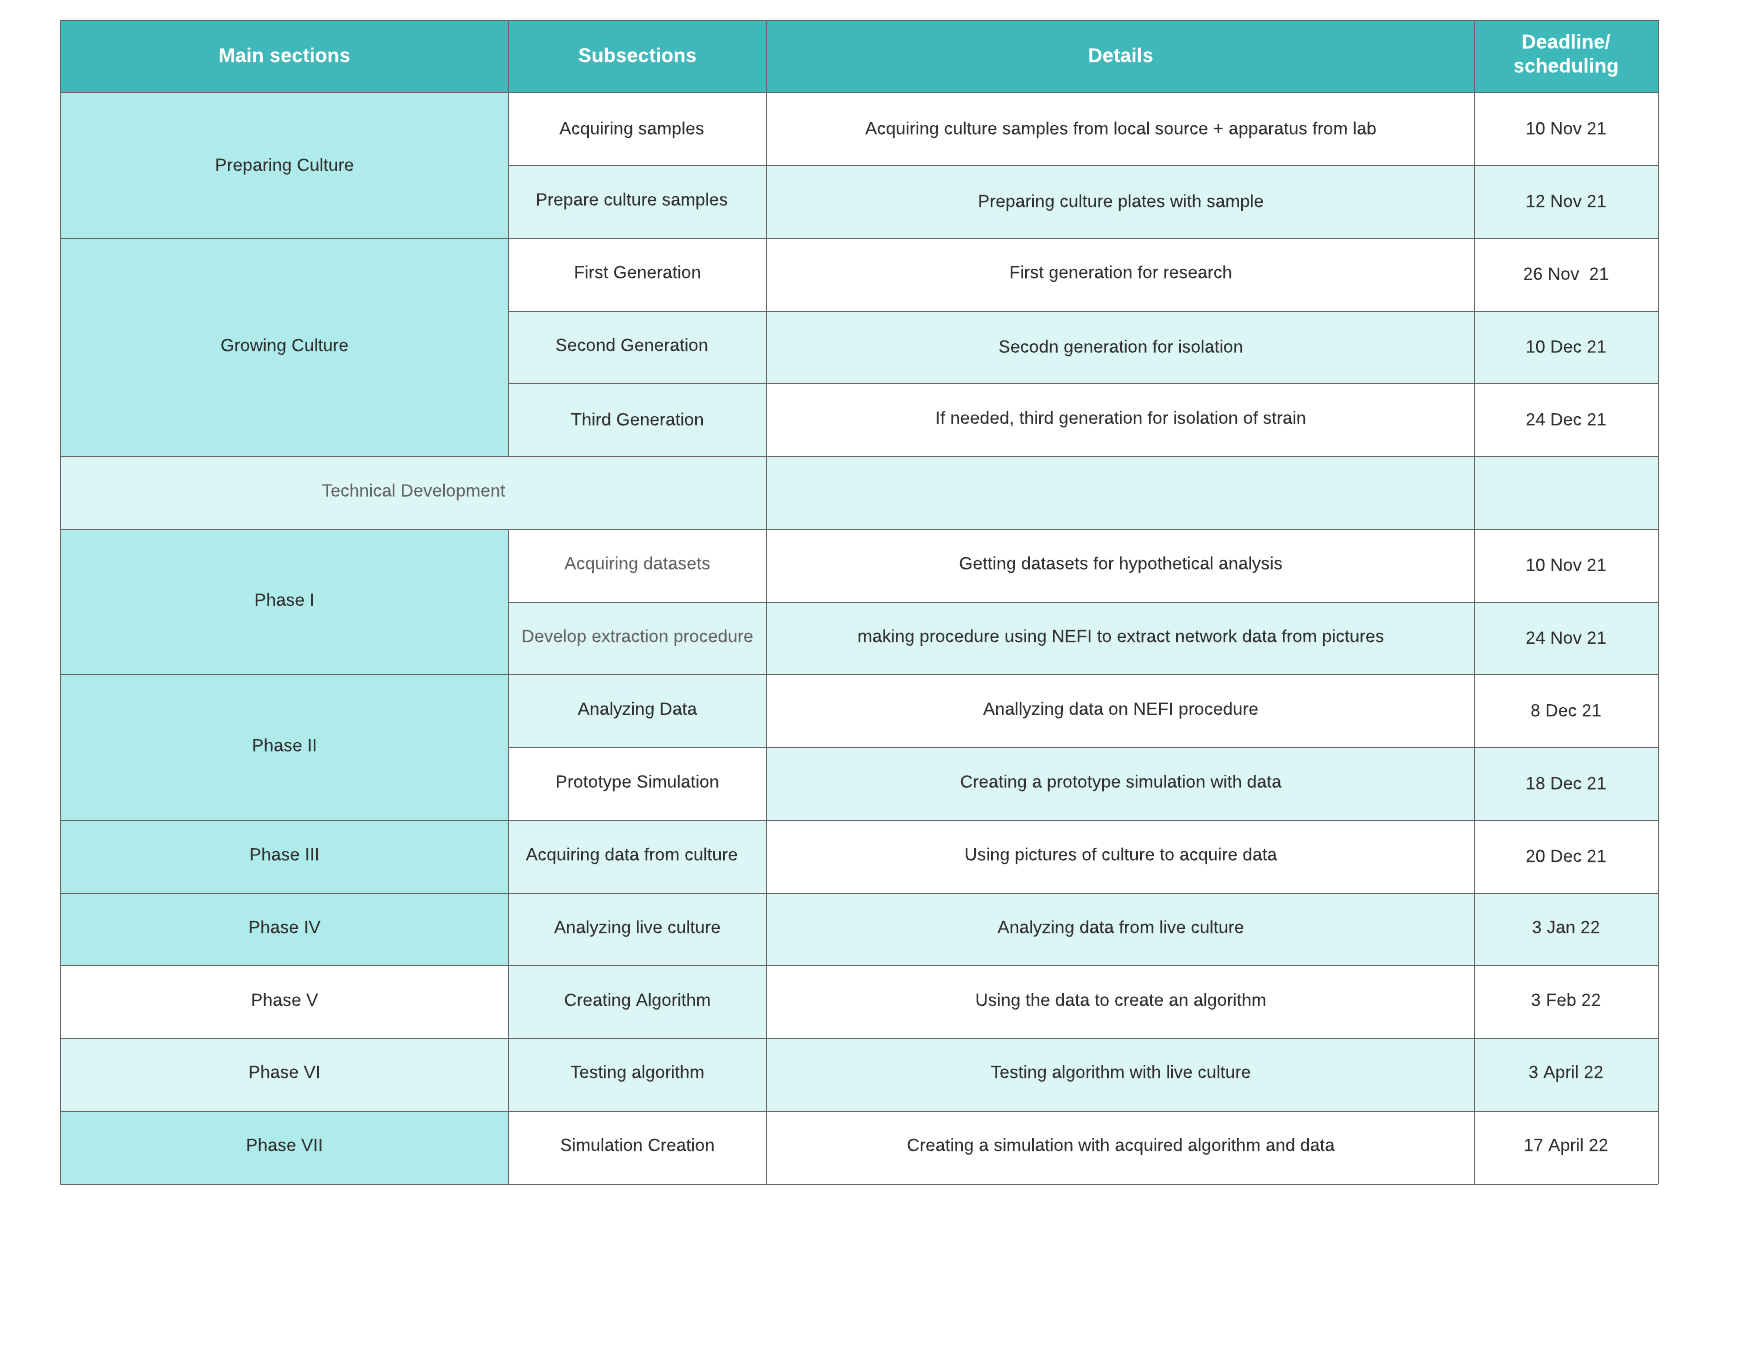
\includegraphics[scale=0.6]{Images/gantt_chart.png}
    \caption{Gantt Chart}
    \label{fig:gantt}
\end{figure}

Deliverables: The approach for our deliverables will be largely adapted from following the procedure for unraveling slime mould intelligence as outlined by Sun
\cite{steiner_tree}.
    
    \begin{enumerate}
        \item Perform experiments revealing mycelium intelligence on agar.
        \item Based on the experimental results, model the mycelium intelligence (algorithm design, heuristic methods, agent-based modelling, etc).
        \item Customize the model for our applications and develop front-end software for running the simulation of our model.
    \end{enumerate}
    
    Note that the approach outlined was for physarum-inspired networking models, but is generalizable to mycelium networks as well.
    
    The following SMART deliverables have been identified by our team:
    
    \begin{itemize}
        \item \textbf{A model of mycelium growth in a generalised environment:} The model will be based on the real behaviour of mycelium as it colonizes an agar plate in search of food. Algorithms, heuristic approach and agent-based models can all potentially be used in this model.
        \item \textbf{Front-end simulation application using the simulation over transport networks for Karachi:} The simulation should have several parameters that can be adjusted, including addition of nodes, changing terrain, and changing environmental conditions. An option for switching between slime mould and oyster mushroom mycelium may also be included in the simulation, to compare and contrast the behaviour of both organisms.
        \item \textbf{Viable mycelium cultures for experimentation in the lab:} Multiple strains will be obtained from grain spawn colonized on agar. From the isolated strains, the ones showing rapid growth, resistance to contamination and temperature fluctuations will be selected. The experiment will be repeated with several mycelium strains for accuracy of results.
        \item A 3D-printed, scaled down model of Karachi's map on an agar plate. This will be the model used for colonization and studying network optimization, as was done in previous experiments \cite{rulesBioDesign} \cite{slimeapprox}
        
    \end{itemize}

\section{Key Challenges}
The following are the key challenges, and their potential solutions (or precautionary measures that may help prevent them), identified by our team.

\paragraph{The Mycelium culture does not survive as long as required}
\mbox{}\\
Grow extra cultures in preparation.

\paragraph{Unforeseen circumstances cause delays in weekly deliverables.}
\mbox{}\\
Exaggerate goals and deadlines in documentation, to allow a buffer-level cushioning at any and every stage of the project.

\paragraph{Hit-by-a-bus Syndrome}
\mbox{}\\
All areas of the project, regardless of who is leading, will be inclusive of participation (and learning, if need be) from all team members. 

\paragraph{Acquiring Datasets}
\mbox{}\\
We plan on reaching out to the first authors of research papers which make use of the same (or similar) data as us, in hopes of acquiring their datasets. Additionally, we also plan to acquire images of a culture with timed intervals to obtain data that we need, using image processing.


\chapter{Literature Review}
\label{chap:lit}
The main paper that we will form a basis of our research is Adamtzky's "Towards a Fungal Computer". \cite{fungalcomp} In the paper, Adamtzky claims that fungi of the genus Basidiomycetes are phenomenologically similar to the slime mold physarum polycephalum. This includes not only the network topology of fungal mycelium, but also its path-finding properties. The author identifies pleurotus ostreatus, i.e. the Oyster mushroom, as a potential candidate for conducting future network science and computing experiments. However, there is currently a gap in the literature of oyster mushroom mycelium and its path-finding properties; the extent to which it is similar to slime mold, and what are the differences, if any. Our research therefore aims to bridge the gaps in this shortage of knowledge by performing experiments that establish the similarity of mycelium to the slime mold.

Another relevant paper is "Rules for Biologically Inspired Adaptive Network Design" \cite{rulesBioDesign} by Tero and others. This paper serves as a foundation for the kind of network science experiments done using physarum polycephalum as a networking agent. We seek to replicate the experiments of this research, but using oyster mushroom mycelium and mapping Karachi's transport network instead of physarum mapping Tokyo's transport network (i.e. subway). The experiment here seeks to replicate a possible map of a subway/underground metro project in Karachi with different terminals, but using a novel agent (pleurotus ostreatus). The end-result of this publication, i.e. producing Minimum Spanning Trees (MSTs) of the optimized network provides a possible outcome for our final experimental results.

The publication "Maze-solving by an
amoeboid organism" \cite{mazesolving} establishes an experimental procedure for maze-solving experiments using Physarum. We will adapt some experimental procedures from this paper to our experiments using oyster mushroom mycelium. Particularly useful to us here is the laboratory setup for creating terrain for the biological agent to colonize.

"Network Organisation of Mycelial Fungi" \cite{networkmyc} is another useful publication which provides an extensive framework for the network representation of physical mycelium as graphs. This includes the adjacency-matrix representation of mycelium as a graph with vertices and edges, comparison of the proposed model with existing solutions (such as the cellular automaton representation of mycelium), as well as some network topology measures (i.e. betweenness centrality) and how they can be applied to mycelial networks. Particularly useful here are some image processing methods for extracting network data from mycelial networks that the authors use in their experimental analysis of live laboratory cultures.

The publication "Physarum can compute shortest paths" \cite{phy_short_path} provides a theoretical framework for mathematically proving the shortest-path finding properties of the slime mold. The authors use an axiomatic approach, modeling flux through the slime mold's capillary tubes and deriving subsequent results from the mathematical model. We intend on using this publication as a basis for deriving a similar result for the path-finding properties of oyster mushroom mycelium.

"Solving the Steiner Tree Problem in Graphs
using Physarum-inspired Algorithms" \cite{steiner_tree} also establishes a heuristic approach to design algorithms for the slime mold's ability to solve the Steiner tree proble; a super-set of the class of problems that include the shortest path problems. The author designs an algorithm using experimental data, building on earlier work in the field and tying experimental results to an actual algorithm. Our research aims to build a similar algorithm, but for Osyter mushroom mycelium rather than the slime mold.

Finally, another publication by Sun, "Physarum-inspired Network Optimization: A
Review" \cite{phy_network_review} provides an overview of the computing and network science experiments using slime molds so far. The experimental approach the author outlines to establish theoretical results from bio-agent data is what we will adapt, but to the oyster mushroom mycelium rather than the slime mold.

We will keep updating this chapter (especially if our project is research-intensive) as our research proceeds and we come across more work related to our problem.

\chapter{Software Requirement Specification (SRS)}
\label{chap:srs}
This chapter provides detailed specifications of the system under development.

% \section{Functional Requirements}

% This section describes each function/feature provided by our system. These functions are logically grouped into modules based on their purpose/users/mode of operations etc (as per our system). A functional hierarchy may look like:
% \begin{outline}
%   \1 Module 1:
%   \2 Function 1:
%   \2 Function 2:
%   \3 Sub Function 1
%   \3 Sub Function 2
%   \1 Module 2:
%   \2 Function 1:
%   \2 Function 2:
%   \1 .........
% \end{outline}

% % --- The above is to be modified as per your project, e.g. a flat list if your system has limited functional requirements.

% \section{Non-functional Requirements}

% This sections mentions the specific non-functional requirements of our system. These generally address performance, scalability, safety, availability, deployment etc.

\section{External Interfaces}

% We expect every project to have at least of the following subsections. This section must be aligned with your project deliverables. Please consult with your project supervisor regarding which of the following section(s) you should include in your report

\subsection{User Interfaces}
The User interface for this project will include a simulation interface built on Netlogo as one of the final deliverables. The user will be able to simulate the growth and optimization of Mycelium networks. This simulation interface will support parameters such as position of food nodes, and starting point of mycelium colonization, among other variables.

\subsection{Application Program Interface (API)}
Images of natural systems might represent patterns of network-like structure, which might reveal vital data regarding the topological properties of the underlying subject. However, the image itself doesn't mechanically offer a proper definition of a network in terms of sets of nodes and edges. Instead, this information ought to be fittingly extracted from the raw image data. Our system will make use of the following libraries for graph acquisition and its analysis; especially in our case where mycelium networks’ data collection relies on images where graph extraction requires domain-specific solutions:
\begin{itemize}
    \item NEFI 2.0: A tool that extracts graphs from images of networks originating in various domains. NEFI provides a completely unique platform permitting practitioners to simply extract graphs from pictures by combining basic tools from image processing, computer vision and graph theory. We anticipate NEFI to enable time-efficient collection of large datasets. It is a flexible toolbox based on a combination of standard image-processing routines. Depending on the characteristics of the input image and therefore the elected pipeline, the standard of the ensuing graph could vary. NEFI's accuracy reflects how closely the computed graph resembles the originally portrayed input network. Thus, once performing segmentation as necessary step in network extraction, NEFI inherits the strengths and the weaknesses of its algorithms.
    \item MathWorks’ Image Processing (IPT) and Computer Vision Toolboxes (CVT): IPT provides a comprehensive set of reference-standard algorithmic programs and advancement apps for image processing, analysis, visualization, and algorithm development. We will perform image phaseation, image enhancement, noise reduction, geometric transformations, image registration, and 3D image processing. Image process tool case apps allow you to automatize common image processing workflows. We will interactively segment image knowledge, compare image registration techniques, and batch-process giant data sets.
    
    CVT provides algorithms, functions, and apps for planning and testing laptop vision, 3D vision, and video processing systems. We will perform object detection and tracking, further as feature detection, extraction, and matching. The tool case provides object detection and segmentation algorithms for analyzing pictures that are overlarge to suit into memory.
    \item NetLogo Py Extension: The general workflow of this extension is to run py:setup py:python to initialize the Python session that NetLogo will talk to, and then use py:run, py:runresult, and py:set to interact with that Python session.
\end{itemize}

\subsection{Hardware/Communication Interfaces}
This project will include a digital image processing phase where we will use images of Mycelium growth taken at timed intervals, to extract the apparent network from these images. This extraction process is going to be supported using \href{http://nefi.mpi-inf.mpg.de}{NEFI 2.0} which is an open-source python tool that allows for extraction of graphical data from images and outputs it in terms of a weighted undirected planar graph. This graphical data will then be used for analysis, and eventually to form the basis for the algorithm to simulate the growth of Mycelium networks.

%\section{Use Cases}
%This section presents detailed use cases of our system.

\section{Datasets}
Our project aims to use datasets representing Mycelium networks in terms of graphs, using an adjacency list or matrix representation. So far we haven't come across an open-source dataset which meets our requirement, however in their paper "Network Organisation of Mycelial Fungi" Fricker and et al. \cite{networkmyc} stored their network data in the form of adjacency matrices which we are hoping to procure from them if feasible (the data remained unpublished). Concurrently, we are also searching for datasets in the form of images of culture growth on agar plates with timed intervals. We can extract such data using NEFI 2.0. 

\section{System Diagram}
This diagram gives a high-level view of the different components of our system and the interactions between them. Each component and the particular tools/technologies/libraries used to build it are described.

\begin{figure}[h!]
    \centering
    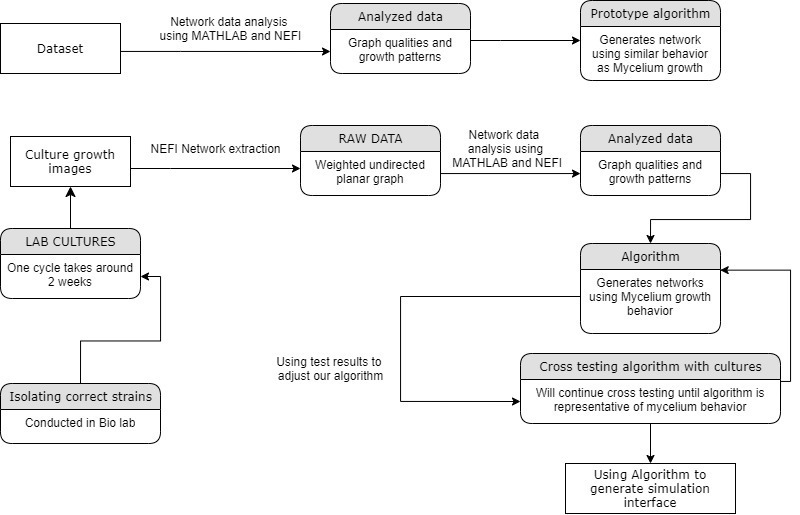
\includegraphics[scale=0.5]{Images/system_diag.png}
    \caption{System Diagram}
    \label{fig:sys_diag}
\end{figure}

\chapter{Software Design Specification (SDS)}
\label{chap:sds}

This chapter provides important artifacts related to design of our project.

\section{Software Design}

This section presents the UML class diagram and gives a brief description of each class in our system. Attributes and methods of each class and relationship among classes are clearly presented.

% Your report will contain ONE of the following 2 sections.

\section{Data Design}

This section presents the structure of our database that caters to persistent data storage in our project. The structure is shown as a normalized data model for relational databases. It clearly shows entities, attributes, relationships with their cardinalities, and primary and foreign keys. We have used DB designer (or any other similar data modeling tool) to build our data model.

 
\section{Technical Details}

Our project does not have persistent data so we have no ERD. Instead we exaplin here the technical details of the algortihsm we use. These include the inputs and the outputs, how and where these algorothms fit in our tool chain, the techniques used in these algorithms, etc.

\chapter{Experiments and Results}
\label{chap:results}
We did many experiments and got the best results.

\chapter{Conclusion and Future Work}
\label{chap:outro}
Our work is awesome. We would write more but we need to catch the flight to collect our Turing Award.

\begin{appendices}

\titleformat{\chapter}[hang]{\bf\huge}{Appendix \thechapter.}{2pc}{}
  
% This appendix is optional.
\chapter{More Math}
Here, we describe the background math for the techniques used in the text.

% This appendix is required if the data set is not fully described in the main text.
\chapter{Data}
Here is a dump of our 2TB data set. Enjoy!

% This appendix is required if the code is not fully described in the main text.
\chapter{Code}
% EITHER dump your code here. No one except HEC likes this.
Here is our code.

% inspired by https://xkcd.com/221/
\begin{lstlisting}[language=python, showstringspaces=false,frame=single]
  print('Hello World!')
  print('Computing true random number.')
  print('Capturing interstellar radiation.')
  print('This will take time!')
  import random
  import time
  time.sleep(3600*random.randint(1,10))
  print(4)
\end{lstlisting}

% OR, link to your GitHub repository. Everyone but HEC will like this.
Our code can be found at \url{https://github.com/habib-university/Kaavish-Template}.

%%% Local Variables:
%%% mode: latex
%%% TeX-master: "../report"
%%% End:

\end{appendices}

% Print the bibliography with a ToC entry and titled, "References".
\printbibliography[heading=bibintoc,title={References}]

\end{document}

%%% Local Variables:
%%% mode: latex
%%% TeX-master: t
%%% End:
